\documentclass{article}
\usepackage{graphicx} % Required for inserting images
\usepackage[margin=1in]{geometry}
\usepackage{amsmath}
\usepackage{amsthm}
\usepackage{amssymb}
\usepackage{amsfonts}
\usepackage{verbatim}
\usepackage{tikz}
\usepackage{xcolor}

\title{Homework 5: Report}
\author{Dante Buhl}


\DeclareMathOperator{\cond}{cond}
\DeclareMathOperator{\vecspan}{span}
\DeclareMathOperator{\sign}{sign}

\begin{document}

\newcommand{\bs}[1]{\boldsymbol{#1}}
\newcommand{\bmp}[1]{\begin{minipage}{#1\textwidth}}
\newcommand{\emp}{\end{minipage}}
\newcommand{\R}{\mathbb{R}}
\newcommand{\C}{\mathbb{C}}
\newcommand{\N}{\mathcal{N}}
\newcommand{\I}{\mathrm{I}}
\newcommand{\K}{\bs{\mathrm{K}}}
\newcommand{\m}{\bs{\mu}_*}
\newcommand{\s}{\bs{\Sigma}_*}
\newcommand{\dt}{\Delta t}
\newcommand{\tr}[1]{\text{Tr}(#1)}
\newcommand{\Tr}[1]{\text{Tr}(#1)}

\maketitle



\section{Numerical Problems}
\begin{enumerate}
    
\item My Tridiagonalization routine successfully makes a square matrix tridiagonal. It really only took a slight modificaiton to my QR decomposition routine and it performs well. Some notes is that machine precision errors will cause the zero's elements to occasionally show a sign. But when I looked at the twonorms of each column in the resulting Tridiagonal form, you find that these values are near machine precision zero (this is investigated by computing the two norms with and without the elements that should be zero and seeing if there is a nontrivial error).

\item My QR algorithms work well and compute the eigenvalues to a high degree of accuracy. The QR with shifts algorithm seems to fail the iteration after the matrix becomes diagonal. I also wrote a print statement tht shows after how many iterations the algorithm converged in. As expected, the algorithm with shifts converges faster. 

\item My inverse iteration method works well. I soon discovered that the order of accuracy of the eigenvectors is limited by the order of accuracy of the eigenvalues. That is, if you give the algorithm an eigenvalue with accuracy out to $10^{-4}$ you can expect your eigenvalues to have an order of accuracy of $10^{-4}$. Because of this, I have my driver routine using QR to compute the eigenvalues out to $10^{-14}$ and my eigenvectors have a great deal of accuracy. 
   
\end{enumerate}


\section{Theory Problems}
\begin{enumerate}

\item %start of problem 1
Consider the Householder matrix defined by
\[
    H = I - 2\frac{vv^T}{v^Tv}
\] 
\begin{enumerate}
\item Show that for any nonzero vector v, the matrix is orthogonal
and symmetric.

\item  Let $a$ be any nonzero vector and let $v = a + \alpha e_1$ , where
$\alpha = \sign(a_{11})||a||_2 $. Show that $Ha = -\alpha e_1$ by direct calculation.

\item Determine $v$ and $\alpha$ that transforms,
\[
    H \left[\begin{array}{c} 1 \\1 \\1\\1\end{array}\right] = \left[\begin{array}{c} \alpha \\0\\0\\0\end{array}\right]
\]
\item Given the vector $a = (2, 3, 4)^T$ , specify a Householder trans-
formation that annihilates the third component of $a$.

\item What are the eigenvalues of $H$ for any nonzero vector $x$?
\end{enumerate}

\begin{enumerate}

\item 
\begin{proof}
Begin by looking at the transpose of H. 
\[
    H^T = \left(\I - 2\frac{vv^T}{v^Tv}\right)^T
\]
\[
    H^T = \I - \frac{2}{v^Tv} (vv^T)^T = \I - 2\frac{vv^T}{v^Tv} = H
\]
So we can immediately see that $H$ is symmetric. Next we look at $H^TH$.
\[
    H^TH = H^2 = \left(\I - 2\frac{vv^T}{v^Tv}\right)\left(\I - 2\frac{vv^T}{v^Tv}\right)
\]
\[
    H^TH = \I - 2\frac{vv^T}{v^Tv} - 2\frac{vv^T}{v^Tv} + \frac{4}{(v^Tv)^2} vv^Tvv^T
\]
\[
    H^TH = \I - 4\frac{vv^T}{v^Tv} + \frac{4 v^Tv}{(v^Tv)^2}vv^T = \I
\]
\[
    H^TH = \I
\]
So we have that $H$ is orthogonal as well. 
\end{proof}


\item 
\begin{proof}
\[ 
    v = a + \alpha e_1, \quad v^T = a^T + \alpha e_1^T
\]
\[
    H = \I - 2\frac{vv^T}{v^Tv} 
\]
\[
= \I - \frac{2}{a^Ta + 2\alpha a_1 + \alpha^2}\left(aa^T + \left[\begin{array}{c}\alpha a^T\\ \hline 0 \\ \hline \vdots \\ 0\end{array}\right] + \left[\begin{array}{c | c | c | c} \alpha a & 0 & \cdots & 0\end{array}\right] + \left[\begin{array}{c c c} \alpha^2 & 0 & \cdots \\ 0  & 0 & \cdots\\ \vdots & \vdots & \ddots\end{array}\right]\right) 
\]
We now multiply by $a$. 
\[
    Ha = a - \frac{2}{a^Ta + 2\alpha a_1 + \alpha^2}\left(aa^Ta + \left[\begin{array}{c}\alpha a^T\\ \hline 0 \\ \hline \vdots \\ 0\end{array}\right]a + \left[\begin{array}{c | c | c | c} \alpha a & 0 & \cdots & 0\end{array}\right]a + \left[\begin{array}{c c c} \alpha^2 & 0 & \cdots \\ 0  & 0 & \cdots\\ \vdots & \vdots & \ddots\end{array}\right]a\right) 
\]
Recall that $a^Ta = \alpha^2$. 
\[
    Ha = a - \frac{2}{\alpha^2 + 2\alpha a_1 + \alpha^2}\left(\alpha^2a + \alpha^3 e_1 + \alpha a_1 a + \alpha^2 a_1 e_1\right) 
\]
\[
    Ha = a - \frac{\alpha}{\alpha(\alpha + a_1)}\left((\alpha + a_1)a + \alpha(\alpha + a_1) e_1\right)
\]
\[
    Ha = a - a - \alpha e_1 = -\alpha e_1
\]
\[
    Ha = -\alpha e_1
\]
\end{proof}

\item
\begin{proof}
    We have evidently that $a = \left[\begin{array}{c} 1 \\ 1\\ 1\\1\end{array}\right]$. Therefore we have that $\alpha = -\sqrt{4}$ and $v = a + \sqrt{4}e_1$. (Note that in this specific case, I am not using $\alpha$ as the exact modifier in the $v$ vector but rather $-\alpha$. 
\[
    v = \left[\begin{array}{c} 1 + \sqrt{4}\\1\\1\\1\end{array}\right]
\]
\end{proof}


\item 
\begin{proof}
    In order to eliminate the third component of $a$ we look for a vector which is equidistant to $a$ and the $x-y$ plane. That way the Householder transformation will project $a$ onto the $x-y$ plane. We will look at a geometrical setup which demonstrates this nicely. Notice for this problem we can cast the vector $a$ into a 2D space in order to simplify this problem. 
    \[
        a = (a_{\zeta}, a_z)^T = (\sqrt{13}, 4)^T, \quad 2^2 + 3^2 = 13 = a_{\zeta}^2
    \]
    Here we have the magnitude of its $\zeta$ component is $\sqrt{13}$ where $\zeta$ is increasing in the direction of $(x, y) = (2, 3)$. We now look to find a vector $x$ such that $d(x, a) = d(x', x)$, where $x'$ is the projection of $x$ onto the $x-y$ plane, and $d(\bs{x_1}, \bs{x_2})$ is the distance function between two points. The congruence of the two triangles created allows us to suppose the magnitude of $x'$ is equal to the norm of $a$ ($||a||_2 = \sqrt{29}$).

    \begin{center}
    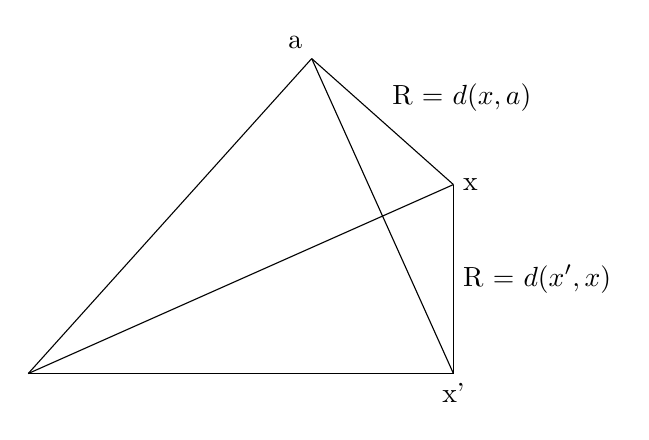
\begin{tikzpicture}

        \coordinate(O) at (0, 0);
        \coordinate(A) at (3.6, 4);
        \coordinate(r1) at (4.5, 3.2);
        \coordinate(r2) at (5.4, 1.2);
        \coordinate(P) at (5.4, 0);
        \coordinate(X) at (5.4, 2.4);
        \draw (O) -- (A);
        \draw (O) -- (X);
        \draw (O) -- (P);
        \draw (A) -- (X);
        \draw (X) -- (P);
        \draw (A) -- (P);
    
        \node[above left] at (A) {a};
        \node[right] at (X) {x};
        \node[above right] at (r1) {R = $d(x, a)$};
        \node[right] at (r2) {R = $d(x', x)$};
        \node[below ] at (P) {x'};
        
    \end{tikzpicture}
    \end{center}

    \[
        R = d(x, a) = \sqrt{(\sqrt{13} - \sqrt{29})^2 + (4 - x_z)^2} = \sqrt{(\sqrt{29} - \sqrt{29})^2 + x_z^2} = d(x', x)
    \]
    \[
        (\sqrt{13} - \sqrt{29})^2 + (4 - x_z)^2 = x_z^2
    \]
    \[
        (\sqrt{13} - \sqrt{29})^2 + 16 = 8x_z
    \]
    \[
        x_z = 2 + \frac{(\sqrt{13} - \sqrt{29})^2}{8} 
    \]
    So we have $x = (x_{\zeta}, x_z)^T = \left(\sqrt{29}, 2 + \frac{(\sqrt{13} - \sqrt{29})^2}{8}\right)$. We go back to a three coordinate system. $x_{\zeta}^2 = x_x^2 + x_y^2$. 
    \[
        x_x = \frac{2}{3}x_y, \quad 29 = x_y^2\left(\frac{4}{9} + 1\right)
    \]
    \[
        x_y = 3\sqrt{\frac{29}{13}}, \quad x_x = 2\sqrt{\frac{29}{13}}
    \]
    So we have, $x = \left(2\sqrt{\frac{29}{13}}, 3\sqrt{\frac{29}{13}}, 2 + \frac{(\sqrt{13} - \sqrt{29})^2}{8}\right)^T$. Finally we look to construct the householder transformation.
    \[
        H = \I - 2\frac{xx^T}{x^Tx}
    \]
    \[
        Ha = a - \frac{2x^Ta}{x^Tx}x
    \]
    \[
        x^Ta = 4\sqrt{\frac{29}{13}} + 9\sqrt{\frac{29}{13}} + 8 + \frac{(\sqrt{13} - \sqrt{29})^2}{2}
    \]
    \[
        x^Ta = \sqrt{13\cdot29} + 8 + \frac{13 + 29}{2} - \sqrt{13\cdot29} = 29 
    \]
    \[
        x^Tx = \frac{4\cdot29}{13} + \frac{9\cdot29}{13} + 4 + \frac{(\sqrt{13} - \sqrt{29})^4}{64} + \frac{(\sqrt{13} - \sqrt{29})^2}{2}
    \]
    \[
        x^Tx = 33 + 21 - \sqrt{13\cdot29} + \frac{(42 - 2\sqrt{13\cdot29})^2}{64}
    \]
    \[
        x^Tx = 54 - \sqrt{13\cdot29} + \frac{7^2\cdot3^2 + 13\cdot19 - 42\sqrt{13\cdot29}}{16}
    \]
    \begin{center}
        \[\mathfrak{One \text{ } ``Trust-me-Bro''\text{ } later...}\]
    \end{center}
    \[
        x^Tx = \alpha, \quad \text{(put the above thing in a calculator to check its right).}
    \]
    \[
        Ha = a - \frac{58}{\alpha}x = \left[\begin{array}{c}-2.987\dotsc \\ -4.480\dotsc \\ 0 \end{array}\right]
    \]
    Actually here is a link to a desmos graph where I have all of the calculations done for me (https://www.desmos.com/calculator/pdxvbhi57x). If you would like to contest it please do. However the proof concludes. This reasoning was based in geometrical argument and used properties of reflection. And through careful calculation, the third component of $a$ is eliminated in one householder transformation. 

\end{proof}

\item
\begin{proof}

To look at the eigenvalues of $H$ we simply look at the definition of an eigenvalue. 
\[
    Hv = \lambda v
\]
\[
   v  - \frac{2x^Tv}{x^Tx}x = \lambda v
\]
\[
    \alpha x = (\lambda - 1) v
\]
Again we have two vectors, not necessarily colinear so we look at the two cases, they are colinear, or they are orthogonal. If they are colinear, $v = cx$ for a constant $c$. 
\[
    -2\frac{x^Tv}{x^Tx}x = c(\lambda - 1)x
\]
\[
    -2c = c(\lambda - 1), \quad \lambda = -1
\]
The other case is that x and v are orthogonal. Notice that then $x^Tv = 0$. 
\[
    0 = (\lambda - 1), \quad \lambda = 1
\]
Thus we have that the eigenvalues of $H$ are $\lambda = -1, 1$.
\end{proof}

\end{enumerate}

\item % start of problem 2
The Schur decomposition theorem states that every square matrix $A\in \C^{m\times m}$ has a Schur Decomposition, $A = QUQ^*$, where $Q$ is a unitary and $U$ is upper triangular. Use this theorem to prove that, for an arbitrary norm $|| \cdot ||$, 
\[
    \lim_{n\to \infty} ||A^n|| = 0 \Longleftrightarrow \rho(A) < 1
\]
(Note: Show the claim first with the 2-norm or the Frobenius norm and use the fact that all norms are equivalent in a finite vector space.)

\begin{proof}

    ($\implies$)

    Let us look at the two-norm of $A^n$. Next we investigate an arbitrary eigenvalue, eigenvector pair of $A$, ($\lambda, v$). We have that, 
    \[
        ||A^n||_2 \ge \frac{||A^nv||_2}{||v||_2} = \frac{|\lambda|^n||v||_2}{||v||_2} = |\lambda|^n 
    \]
    We go back to the limit as $n \to \infty$. 
    \[
        \lim_{n \to \infty} ||A^n||_2 = 0 > |\lambda|^n
    \]
    Therefore we have that $|\lambda| < 1$. Since this observation is independent of which p-norm is chosen and which eigenvalue of $A$ we chose, we must have that all eigenvalues of $A$ are such that $|\lambda| < 1$ and therefore we must have that $\rho(A) < 1$. 
    

    ($\impliedby$) 

    Given that for a matrix $A = QUQ^*$ and $\rho(A) < 1$. We have that the eigenvalues of $A$ are along the diagonal of $U$ (Mini proof: $A$ is similar to $U$, and $\det(U - \lambda I) = \Pi_{i=1}^m (u_{ii} - \lambda)$ since $U$ is upper triangular. Therefore the eigenvalues of $U$ are found along its diagonal.)  Next since $\rho(A) < 1$ we have that all of the eigenvalues of $A$ are of absolute value less than 1. So we have that,
\[
    \lim_{n\to \infty} ||A^n|| = \lim_{n\to \infty} ||QU^nQ^*|| = \lim_{n\to \infty} ||U^n||
\] 
Now to show that the norm is equal to zero irrespective of which norm is taken, we need to show that $U^n \to 0$. This requires induction. We start with the base case: that the diagonal goes to zero. We have that the diagonal is constructed of the eigenvalues of $A$ which are all less than 1 in absolute value. We look at the matrix product $U^2$. 
\[
    U^2 = UU = \left[\begin{array}{ c c c} \lambda_1^2 & u_{12}(\lambda_1 + \lambda_2) & \cdots \\ 
                                            0 & \lambda_2^2  & \cdots \\ \vdots & \vdots & \ddots \end{array}\right]
\]
Notice that the diagonal entries of $U^n$ will be $u_{ii} = \lambda_i^n$. Since all $|\lambda_i| < 1$ we have that $\lambda^n \to 0$ as $n \to \infty$ or rather $\lambda^n \approx 0$ as $n$ becomes large but still finite. So we have the the diagonal will tend towards zero as $n$ increases. Our inductive step is then to look at $U$ described as the following. $U_k = \left[\begin{array}{c c} \bs{0} & R_k \\ \bs{0} & \bs{0} \end{array}\right]$. Here $R_k$ is an upper triangular matrix, $R_k \in \R^{m-k\times m-k}$. Our goal is to show that by multiplying by $U$ some discrete amount of times, that we will find $U_{k+1}$ where, $U^{k+1} = \left[\begin{array}{c c} \bs{0} & R_{k+1} \\ \bs{0} & \bs{0} \end{array}\right]$ and $R_{k+1} \in \R^{m-k-1\times m - k -1}$. That is, the diagonal of $R_k$ will go to zero, producing $R_{k+1}$ inside of it. We begin, 
\[
    U_kU = \left[\begin{array}{ c c c c} 
                \bs{0} & r_{11}\lambda_k & \cdots & \cdots\\ 
                \bs{0} & 0  & r_{22}\lambda_{k+1} & \cdots  \\
                \vdots & \vdots & \vdots  & \ddots \end{array}\right]
\]
We can see that if we multiply by $U$ by a finite amount of times, we will eventually obtain similarly that $U_kU^n$ which has zeros on what used to be the diagonal of $R_k$ (the diagonal of $R_k$ will be multiplied by its respective $\lambda$ some amount of times such that, $r_{jj}\lambda_{k+j}^n \to 0$ as $n \to \infty$. Notice that for some smaller, finite $n$ we will have $r_{jj}\lambda_{k+j}^n \approx 0$. Therefore after multiplying by some finite number of $U$ we will effectively obtain $U_{k+1}$ which has the following form $U_{k+1} = \left[\begin{array}{c c} \bs{0} & R_{k+1} \\ \bs{0} & \bs{0} \end{array}\right]$ and $R_{k+1} \in \R^{m-k-1\times m - k -1}$. Notice that this is effectively done with finite multiples of $U$. That is, $U_{k+1} = U^n$ such that $n < \infty$. 

The inductive step is complete! If we have $U_k$ from finite multiples of $U$, through additional finite multiples of $U$ we obtain $U_{k+1}$. Therefore, we return to the limit and obtain the matrix $U_m$ which with all intents and purposes is an $m\times m$ zero matrix to machine precision. 
    \[
        \lim_{n\to \infty} ||A^n|| = \lim_{n\to\infty} ||U^n|| = ||U_m||
    \]
    Finally we have that a zero matrix has norm of zero. 
    \[
        \lim_{n\to\infty} ||A^n|| = ||U_m|| = ||\bs{0}|| = 0
    \]
    
\end{proof}

\item   % start of problem 3
Let $A \in \C/\R^{m\times n}$ and $B \in \C/\R^{n \times m}$. Show that the matrices $\left[\begin{array}{c c} AB & 0 \\ B & 0\end{array}\right]$ and $\left[\begin{array}{c c} 0 & 0 \\ B & BA \end{array}\right]$ have the same eigenvalues. 

\begin{proof}
   
    We start by looking at the determinant of block matrices. Take for example the matrix $\Gamma = \left[\begin{array}{c c} A & B \\ 0 & D\end{array}\right]$.
    \[
        \Gamma = \left[\begin{array}{c c} \I & 0 \\ 0 & D \end{array}\right]\left[\begin{array}{c c} \I & B \\ 0 & \I \end{array}\right] \left[\begin{array}{c c} A & 0 \\ 0 & \I\end{array}\right]
    \]
    We look at the determinant of $\Gamma$. 
    \[
        \det(\Gamma) = \det\left(\left[\begin{array}{c c} \I & 0 \\ 0 & D \end{array}\right]\right)\det\left(\left[\begin{array}{c c} \I & B \\ 0 & \I \end{array}\right]\right)\det\left(\left[\begin{array}{c c} A & 0 \\ 0 & \I \end{array}\right]\right)
    \] 
    \[
        \det(\Gamma) = \det(D)\det(A)
    \]
    The same is obviously true for a matrix $\Gamma$ of the form, $\Gamma = \left[\begin{array}{c c} A & 0 \\ B & D\end{array}\right]$ with $A$ invertible \[\Gamma = \left[\begin{array}{c c} \I & 0 \\ BA^{-1} & \I \end{array}\right]\left[\begin{array}{c c} \I & 0 \\ 0 & D \end{array}\right] \left[\begin{array}{c c} A & 0 \\ 0 & \I\end{array}\right]\]
. We now look at the eigenvalues of $M_1 = \left[\begin{array}{c c} AB & 0 \\ B & 0\end{array}\right]$ and $M_2 = \left[\begin{array}{c c} 0 & 0 \\ B & BA \end{array}\right]$. We look at the determinants, 
    \[
        \det(M_1 - \lambda \I) = \det(AB - \lambda \I)\det(-\lambda \I)
    \]
    \[
        \det(M_2 - \lambda \I) = \det(-\lambda \I)\det(BA - \lambda \I)
    \]
    Notice that if $\lambda$ is an eigenvalue of its respective matrix then this determinant product must be equal to zero. We then take the case of each determinant can be zero. For $M_1$ we have that its eigenvalues are either zero, or the eigenvalues of $AB$ by definition. 
    \[
        \det(M_1 - \lambda \I) = 0, \quad \det(AB - \lambda \I) = 0,\quad  \det(-\lambda \I) = -\lambda = 0
    \]
    Similarly we have that the eigenvalues for $M_2$ are either zero or the eigenvalues of $BA$. Notice from a different homework problem (hw2), we have that the matrix products $AB$ and $BA$ have the same eigenvalues. This is because, 
    \[
        ABv = \lambda v, \quad Bv = y, \implies \quad BAy = \lambda y
    \]
    Finally both $M_1$ and $M_2$ have eigenvalues of zero and the eigenvalues of $AB/BA$. 
    
\end{proof}


\item % start of problem 4
Show that for a real-valued square matrix the Gerschgorin theorem also holds with the bounds $r_i$ which are given by the partial column sums (instead of the partial row sums):
\[
    r_i = \sum_{i=1, i\neq j}^m |a_{i,j}|, \quad i = 1, \dots, m
\]

\begin{proof}
    We begin by reviewing Gershgorin's Theorem. We have for a square matrix $A$. It's eigenvalues are bound by the row sums along $A$. That is,
    \[
        |\lambda - a_{ii}| \le \sum_{j = 1, j \neq i}^m |a_{ij}|
    \]
    We now look at some properties of $A$. We have that since $\det(A) = \det(A^T)$ for real matrices $A$ that, $\det(A - \lambda\I) = \det(A^T + \lambda\I^T) = \det(A^T - \lambda\I)$. We notice that $A$ and $A^T$ have the same eigenvalues. We next apply Gershgorin's theorem for $A^T$. We find, 
    \[
        |\lambda - a_{ii}| \le \sum_{j=1, j\neq i}^m |a_{ji}|
    \]
    Notice that we have, 
    \[
        |\lambda - a_{ii}| \le \sum_{j = 1, j \neq i}^m |a_{ij}|, \quad |\lambda - a_{ii}| \le \sum_{j=1, j\neq i}^m |a_{ji}|
    \]
    \[
        |\lambda - a_{ii}| \le \min\left\{\sum_{j=1, j\neq i}^m |a_{ij}|, \sum_{j=1, j\neq i}^m |a_{ji}|\right\}
    \]
    That is, Gershgorin's Theorem applyies for the column sums as well in addition to the row sums and often you can minimize the radius by picking the lower of the column or row sum. 
\end{proof}


\item  % start of problem 5
Use the Gerschgorin theorem to show that the following matrix has exactly one eigenvalue in each of the four circles: $|z - k| \le 0.1, \quad k = 1, 2, 3, 4$. 
\[
    A = \left[\begin{array}{c c c c} 1.0 & 0.3 & 0.1 & 0.4 \\
                                    0.0 & 2.0 & 0.0 & 0.1 \\
                                    0.0 & 0.4 & 3.0 & 0.0 \\
                                    0.1 & 0.0 & 0.0 & 4.0 \end{array}\right]
\]

\begin{proof}
    
    We simply apply Gershgorin's Theorem. 
    \[
        |\lambda_1 - 1.0| \le \min\left\{\sum_{j=1, j\neq 1}^m |a_{1j}|, \sum_{j=1, j\neq 1}^m |a_{j1}|\right\}
    \]
    \[
        |\lambda_2 - 2.0| \le \min\left\{\sum_{j=1, j\neq 2}^m |a_{2j}|, \sum_{j=1, j\neq 2}^m |a_{j2}|\right\}
    \]
    \[
        |\lambda_3 - 3.0| \le \min\left\{\sum_{j=1, j\neq 3}^m |a_{3j}|, \sum_{j=1, j\neq 3}^m |a_{j3}|\right\}
    \]
    \[
        |\lambda_4 - 4.0| \le \min\left\{\sum_{j=1, j\neq 4}^m |a_{4j}|, \sum_{j=1, j\neq 4}^m |a_{j4}|\right\}
    \]

    \[
        |\lambda_1 - 1.0| \le 0.1
    \]
    \[
        |\lambda_2 - 2.0| \le 0.1
    \]
    \[
        |\lambda_3 - 3.0| \le 0.1
    \]
    \[
        |\lambda_4 - 4.0| \le 0.1
    \]
    Since the circles don't overlap, we have that $A$ has four non-zero eigenvalues one within each of the circles described above. 


\end{proof}


\item %start of problem 6
Let $A \in \R^{m \times m}$ be real and symmetric that is positive definite. Let $y \in \R^m$ be nonzero. Prove that the limit exists and is an eigenvalue of $A$.
\[
    \lim_{k \to \infty} \frac{y^TA^{k+1}y}{y^TA^ky}
\]

\begin{proof}
    First, since $A$ is real and symmetric, we can decompose $A$ into an eigenvector matrix, full with orthonormal eigenvectors which form a basis for $\R^m$ and a diagonal matrix with eigenvalues of $A$ on the diagonal. Since its columns form a basis for $\R^m$ we have that we can express y as a linear combination of the eigenvectors of v: $y = c_1 v_1 + \cdots + c_m v_m$. We now define $\lambda_*$ such that, $|\lambda_*| \ge |\lambda_i|, \forall \lambda_i \in \Lambda(A), c_* \neq 0$.  
\[
    A = VDV^{-1}, \quad y = c_* v_* + c_1 v_1 + \cdots + c_m v_m
\]
\[
    A^n = VD^nV^{-1},\quad A^ny = c_*\lambda_*^n v_* + c_1\lambda_1^nv_1 + \cdots + c_m\lambda_m^nv_m
\]
\[
   A^ny = \lambda_*^n\left(c_* v_* + c_1\frac{\lambda_1^n}{\lambda_*^n} v_1 + \cdots + c_m\frac{\lambda_m^n}{\lambda_*^n}v_m\right)
\]
Note from our definition of $\lambda_*$ we either have that $|\lambda_*| \ge |\lambda_i| \bigvee \left(|\lambda_* < |\lambda_i| \bigwedge c_i = 0\right)$. Thereby, we have that 
\[
    \lim_{n\to \infty} A^ny = \lambda_*^nc_*v_*
\]
Therefore we have, 
\[
    \lim_{k \to \infty} \frac{y^TA^{k+1}y}{y^TA^ky} = \frac{\lambda_*^{k+1} c_* y^Tv_*}{\lambda_*^k c_* y^Tv_*} = \lambda_*
\]
Where $\lambda_*$ is the largest eigenvalue of $A$ which has an eigenvector as part of the expansion of $y$ into the basis of the eigenvectors of $A$. 
\end{proof}


\item % start of problem 7
Let $A \in \R^{m\times m}$ be real with nonnegative entries such that 
\[
    \sum_{j=1}^m a_{ij} = 1 \quad (1\le i \le m)
\]
Prove that no eigenvalue of $A$ has an absolute value greater than 1.

\begin{proof}
    
    We start by looking at an arbitrary p-norm of the matrix product of $A$ and one of its eigenvectors. 
    \[
        Av = \lambda v, \quad ||Av|| = ||\lambda v||
    \]       
    \[
        ||Av|| \le ||A||||v||, \quad |\lambda|||v|| \le ||A||||v||
    \]
    \[
        |\lambda| \le ||A||
    \]
    We obtain the following inequality which is satisfied by any p-norm we would like to take. We simply chose $p=1$, the one norm. By definition of the one norm for matrices (lecture 5 notes) we have, 
    \[
        |\lambda| \le ||A||_1 = \max_{i} \sum_{j=1}^m a_{ij} 
    \]
    We also have that $A$ is given such that its row sum along any row will sum to 1. Therefore we have,
    \[
        |\lambda| \le ||A||_1 = 1, \implies |\lambda| \le 1
    \]

\end{proof}

\item %start of problem 8
Let $A \in \R^{m\times m}$ be a non-defective matric with its eigenvalues $\{\lambda_i\}_{i=1}^m$ and its singular values $\{\sigma_i\}_{i=1}^m$, satisfying
\[
    |\lambda_1| \ge |\lambda_2| \ge \cdots \ge |\lambda_m|
\]
\[
    \sigma_1 \ge \sigma_2 \ge \cdots \ge \sigma_m
\]
Let $\rho(a)$ be the spectral radius of $A$ and $\cond(A) = ||A||_2||A^{-1}||_2$ be the condition number of $A$. Let $A$ be normal, i.e., $A^TA = AA^T$. Show that: 
\begin{enumerate}
\item $\sigma_i = |\lambda_i|, 1 \le i \le m$.

\item $||A||_2 = |\lambda_1| = \rho(A)$. 
\end{enumerate}

\begin{enumerate}

\item 
\begin{proof}
    We begin with the fact that $A$ is non-defective, is normal, and then has a Singular Value Decomposition. First we look at a diagonalization of $A$ by fact that $A$ is non-defective. 
    \[
        V^{-1}AV = D_{\lambda} \implies A = V_{\lambda}D_{\lambda}V_{\lambda}^{-1}
    \]
    Notice that since, $A$ is non-defective, $A$ the eigenvalues of $A$ form a basis for $\R^m$ (i.e. $V_{\lambda}$ is orthogonal). More importantly, as a given in the diagonalization $V_{\lambda}$ is invertible. 
    \[ 
        V^TV = \I, \implies  V^TVV^{-1} = V^{-1}, \implies  V^T = V^{-1}
    \]
    \[
        A^TA = V^{-T}DV^TVDV^{-1} = VD^2V^{-1} = A^2
    \]
    We also have that $A$ is invertible since it is nondefective. So we find that $A$ is symmetric. 
    \[
        A^TAA^{-1} = A^2A^{-1} \implies A^T = A
    \]
    At this point we can reference Theorem 5.5 of the textbook (on page 45 or 44 of the pdf). The rest of the proof follows. The logic cited there states is to take $A = VDV^{-1}$ where $V^T = V^{-1}$ and then to create a matrix $S_{\lambda}$ which is a diagonal  ``sign'' matrix with only the signs of each eigenvalue on $D$ in the diagonal. That is we can decompose $D = S_{\lambda}|D|$. We then write
    \[
        A = VS_{\lambda}|D|V^{-1}
    \]
    Notice that since $V$ is orthogonal, so is $VS_{\lambda}$, and alternatively $V^T$ was already orthogonal. Then notice that $|D|$ is a positive definite diagonal matrix. Hence we have that $U = VS_{\lambda}$ , $\Sigma = |D|$, and $V^T = V^{-1}$ is a valid SVD of $A$. Therefore we have that the singular values of $A$ are $\sigma_i = |\lambda_i|$ with the implicit scaling (ordering of $\lambda_i$) $|\lambda_1| \ge |\lambda_2| \ge \dotsc \ge |\lambda_m|$.

\end{proof}

\item
\begin{proof}
    If it is given that for a matrix $A$ that is a square, normal, and non-defective matrix, we have that $\sigma_i = |\lambda_i|, \forall i, 1 \le i \le m$. Note that both $\sigma_i$ and $|\lambda_i|$ monotonically decrease as $i$ increases in this particular problem.  Therefore we then look at the two-norm of $A$. We have from some lecture note (probably lecture 5) the following property of the two-norm. $||A||_2 = \sigma_1$. Then we also have that as a given and by definition of the spectral radius of $A$, $\rho(A) = |\lambda_1|$, the largest eigenvalue of $A$.
    \[
        ||A||_2 =  \sigma_1 = |\lambda_1| = \rho(A)
    \]
\end{proof}

\end{enumerate}



\end{enumerate}

\end{document}
